\documentclass{beamer}

\usepackage{amsmath,amssymb,amsthm}
\usepackage{algorithm,algorithmic}
\usepackage{CJK}
\usepackage{txfonts}
\usepackage{subfigure}
\usepackage{pgf,tikz}
\usepackage{changepage}

\usetikzlibrary{shapes,arrows,automata}
\setbeamercovered{transparent}

\newtheorem{thm2}{Theorem}[section]
\newtheorem{remark}[thm2]{Remark}
\newcommand{\Pow}{\mathbf{P}}

%\usetheme{Warsaw,Antibes,Madrid,JuanLesPins,bars}
\usetheme{CambridgeUS}
%\usetheme{Hannover,Singapore}
\begin{document}
\begin{CJK}{GBK}{kai}

    \title[Context-Aware Event Recommendation]{Context-Aware Event Recommendation in
            Event-Based Social Networks \,(RecSys 2015\,) \\
            \vspace{0.2cm} 
            {\color{black}\small{Augusto Q. Macedo, Leandro B. Marinho and Rodrygo L. T. Santos}}}
    \institute[ECNU]{Department of Computer Science, East China Normal University}
    \author[TIAN Jun Feng]{TIAN Jun Feng \quad (��~����)}
    \date{\today}
    \frame{\titlepage}

\section{Outlines}

\frame{\frametitle{Event-Based Social Networks\,(EBSNs\,)}
People can create events of any kind and share it with other users.

\begin{figure}[h]
\centering
{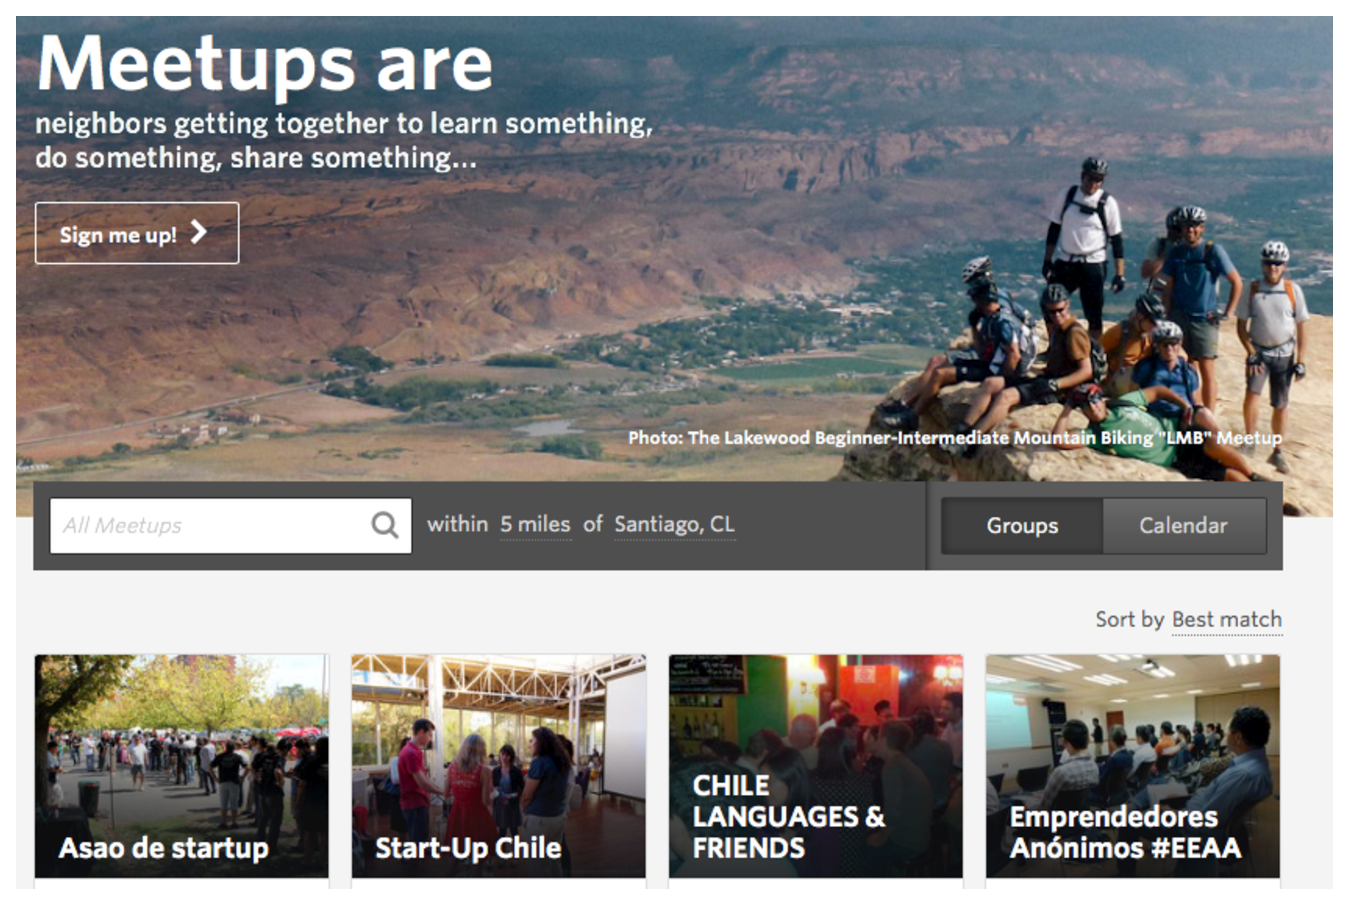
\includegraphics[width=0.70\columnwidth]{figs/3.eps}}
\\
{\centering{Which events best match the user's preferences?}}
\end{figure}
}

\frame{\frametitle{Outline}

\begin{itemize}
\item Problem Setting and Motivation
\vspace{0.3cm}
\item Contextual Models\,(Social, Content, Location, Time\,)
\vspace{0.3cm}
\item Experimental and Evaluation
\vspace{0.3cm}
\item Conclusions
\end{itemize}
}

\section{Motivation}
\frame{\frametitle{Problem}
Event Recommendation is Intrinsically \textbf{Cold-Start}
\begin{figure}[h]
\centering
{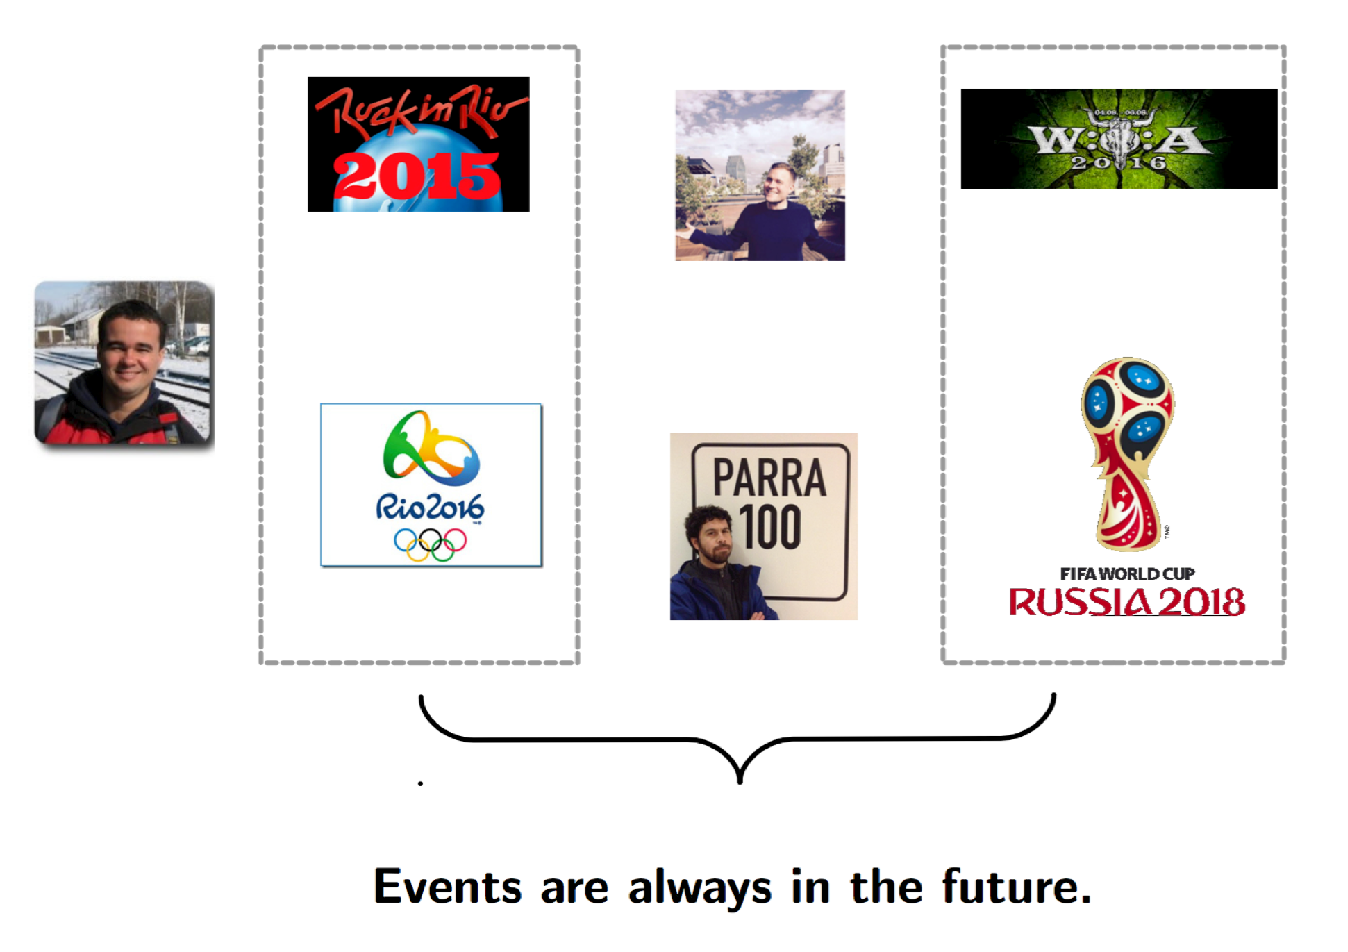
\includegraphics[width=0.82\columnwidth]{figs/figsss/11.eps}}
\end{figure}
}

\frame{\frametitle{Idea 1: Use RSVP as a Proxy for Event Attendance}
{\color{blue}RSVP}: "please respond". After the creation of a public event, any user can RSVP
to it with "yes" or "no".
\begin{figure}[h]
\centering
{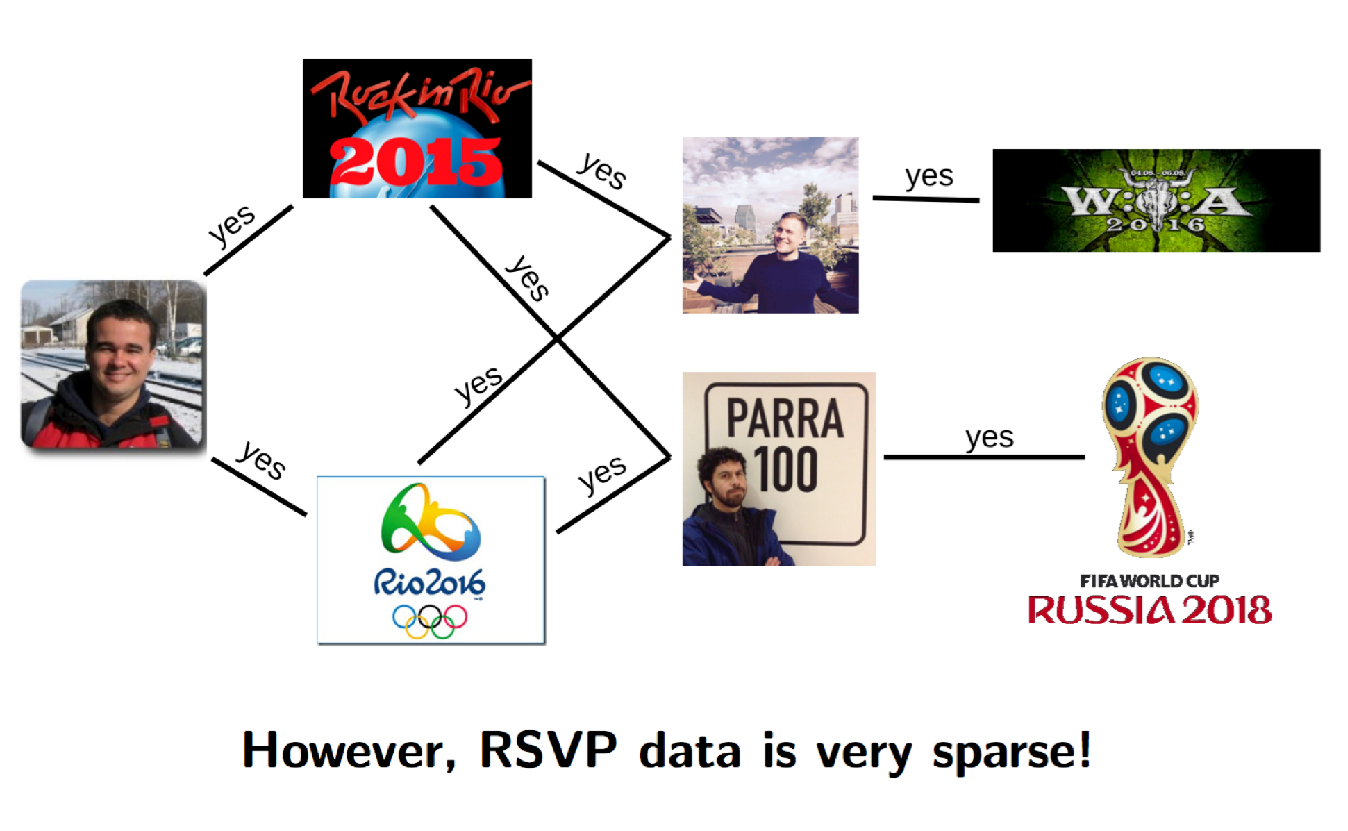
\includegraphics[width=0.82\columnwidth]{figs/figsss/12.eps}}
\end{figure}
}

\frame{\frametitle{Sparsity Level per User}
\begin{figure}[h]
\centering
{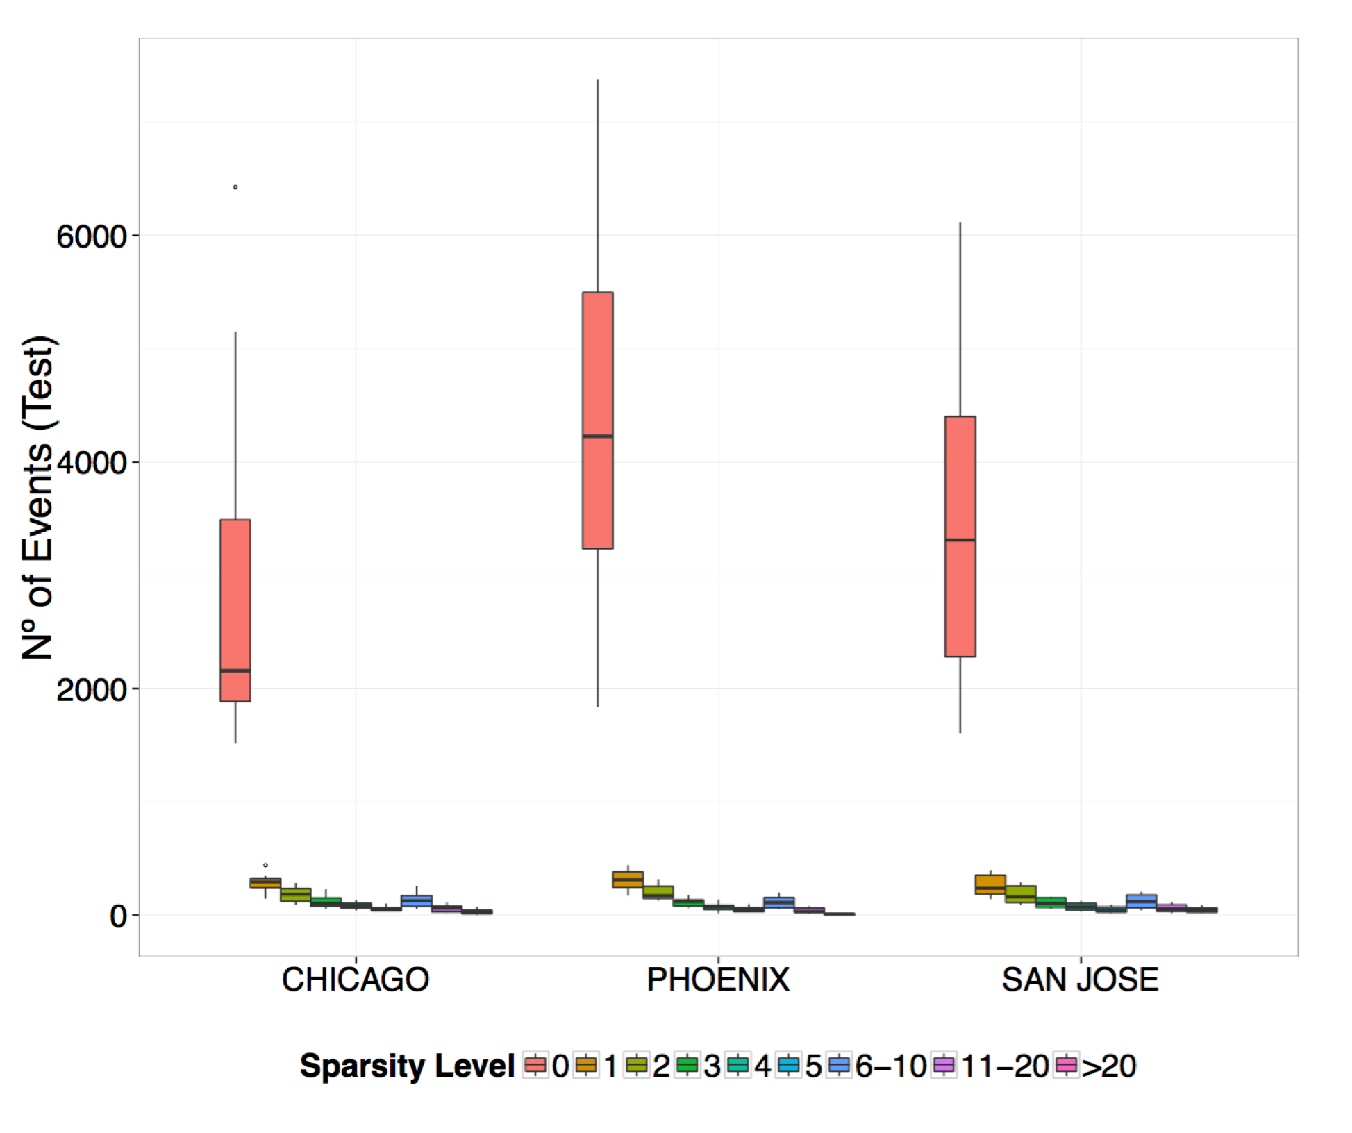
\includegraphics[width=0.72\columnwidth]{figs/figsss/13.eps}}
\end{figure}
}

\frame{\frametitle{Idea 2: Use Contextual Data}
\begin{figure}[h]
\centering
{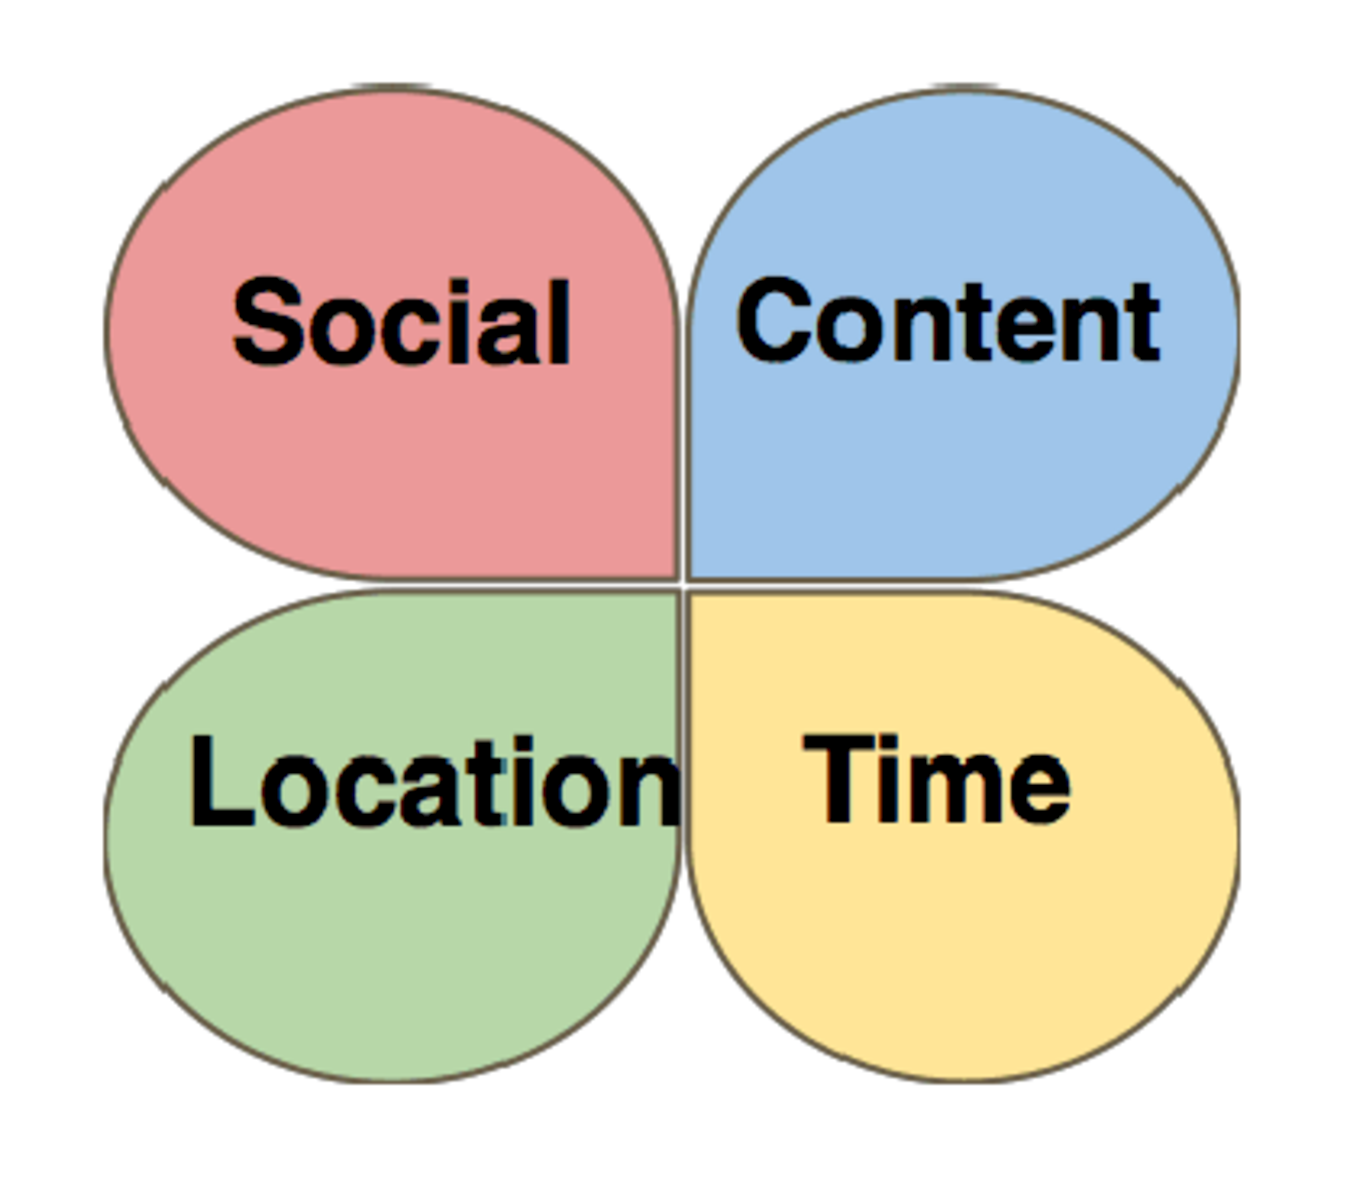
\includegraphics[width=0.6\columnwidth]{figs/figsss/1444.eps}}
\caption{Multi-Contextual Learning to Rank Events (MCLRE)}
\end{figure}
}

\section{Contextual Models}

\subsection{Social-Aware}
\frame{\frametitle{Social-Aware: Group Frequency}
\begin{columns}
\column{0.5\textwidth}
The more events a user attends in a group, the higher the probability he will attend a new
event of this group. Formally:
$$\hat{s}(u, e) := \frac{|E_{u,g_e}|}{E_u}$$

\column{0.5\textwidth}
\begin{figure}[h]
\centering
{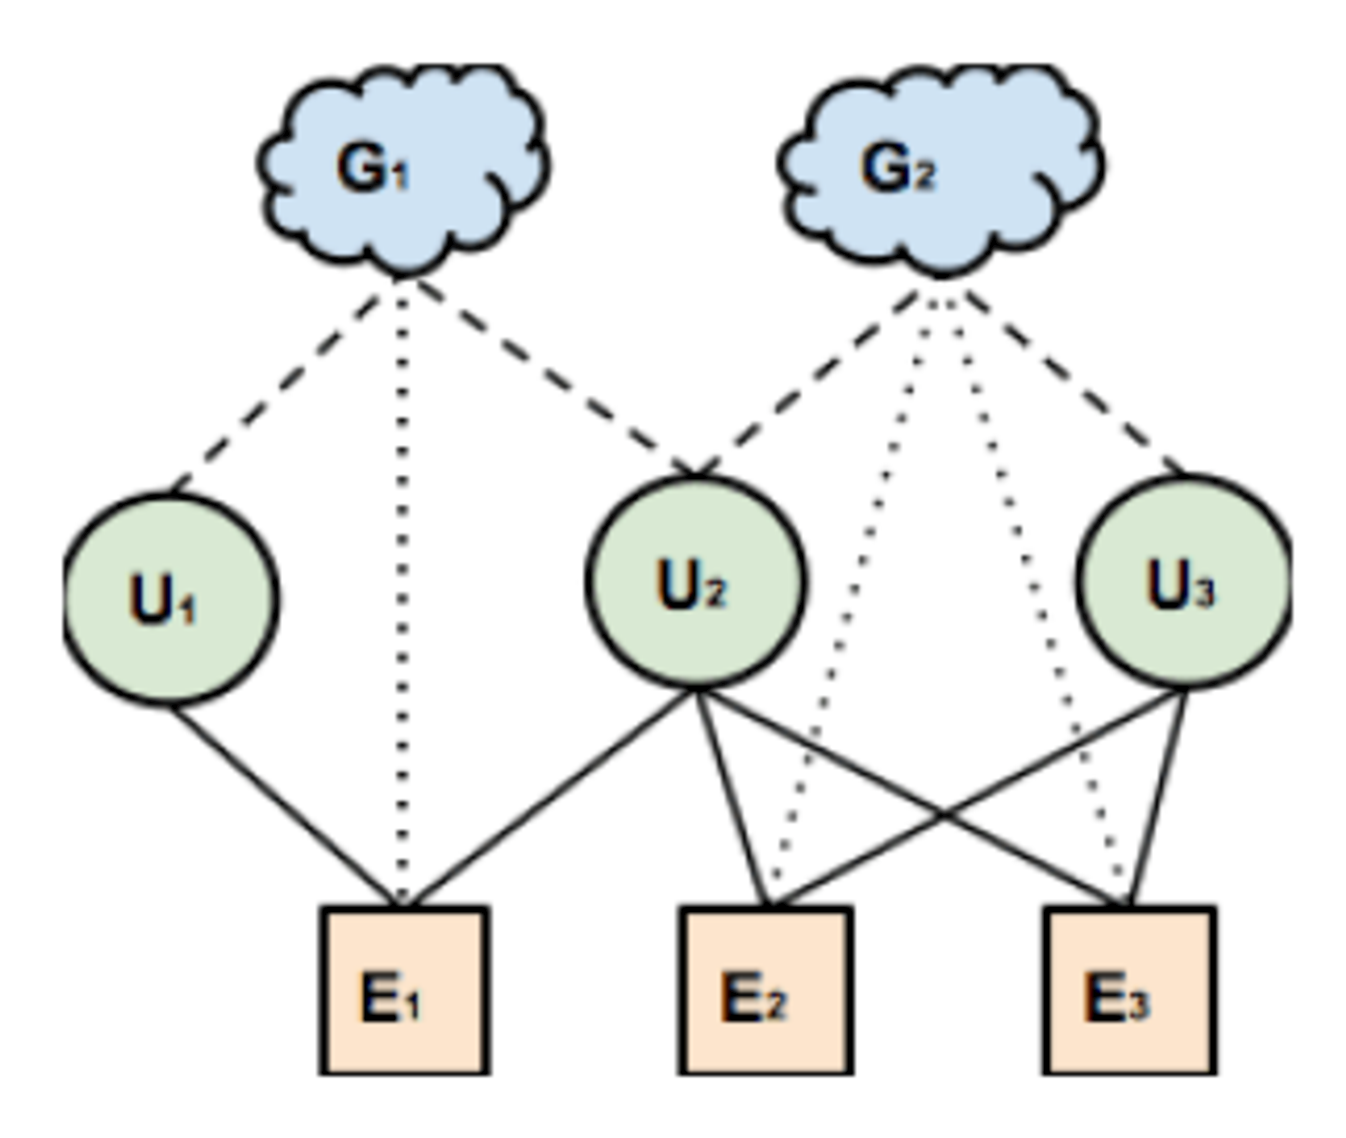
\includegraphics[width=0.8\columnwidth]{figs/figsss/1311.eps}}
\end{figure}
\end{columns}
}

\frame{\frametitle{Multi-Relational Matrix Factorization [Drumond, 2012]}
{\setlength\arraycolsep{2pt}
\begin{eqnarray}
argmin_{\Theta} & \underbrace{\alpha L(R_{UE}, UE^T) + \beta L(R_{UG}, UG^T) + \gamma L(R_{GE}, GE^T)}_{\textrm{sum of weighted losses}}{}
\nonumber\\
& {} \underbrace{ + \lambda_U \parallel U \parallel + \lambda_E \parallel E \parallel + \lambda_G \parallel G \parallel}_{\textrm{regularization term}}
\end{eqnarray}}
\begin{itemize}
\item $R_{XY}\ldots$ Relation between $X$ and $Y$.
\item $\Theta := \{U, E, G\}\dots$ latent matrices of U, E, G resp.
\item $L \ldots$ BPR loss function.
\end{itemize}
\vspace{0.5cm}
The recommendation score is given by:
$$\hat{s}(u,e) = \sum\limits_{f = 1}^{k}\vec{u_f}\vec{e_f}$$
}


\subsection{Content-Aware}

\frame{\frametitle{Content-Aware}
{\color{blue}Content} may help to capture similar and recurrent events.
\begin{figure}[h]
\centering
{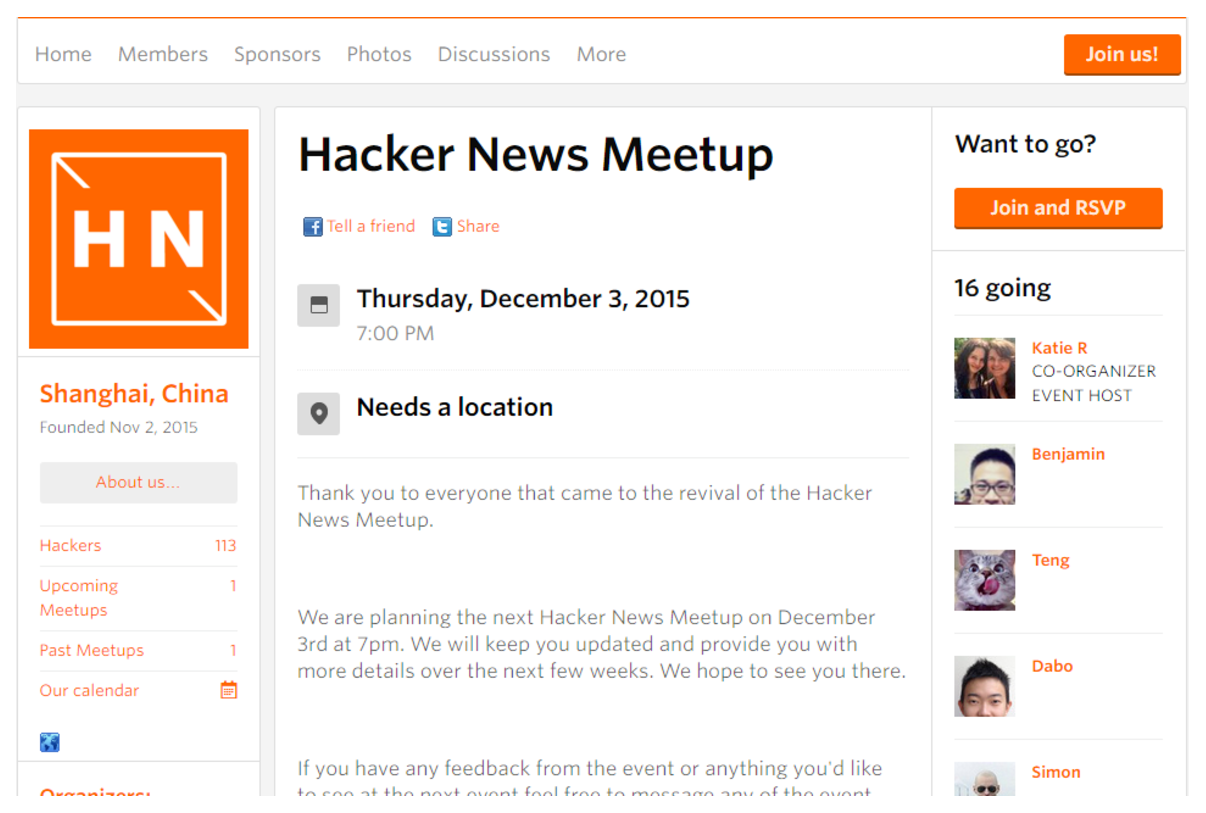
\includegraphics[width=0.7\columnwidth]{figs/2.eps}}
\end{figure}
}

\frame{\frametitle{TF-IDF with time decay}
User profile is the aggregation of all her events' TF-IDFs weighted:
$$\vec{u} := \sum\limits_{e \in E_u} \frac{1}{(1+\alpha)^\tau} \times \vec{e}.$$
\begin{itemize}
\item $\vec{e}\ldots$TF-IDF of event $e$.
\item $\alpha\ldots$time decay factor.
\item $\tau(e)\ldots$days from the RSVP to e until the recommendation moment.
\end{itemize}
\vspace{0.5cm}

The recommendation score is given by:
$$\hat{s}(u, e) = cos(\vec{u}, \vec{e}).$$
}


\subsection{Time-Aware}
\frame{\frametitle{Which time do users go to events?}
\begin{figure}[h]
\centering
{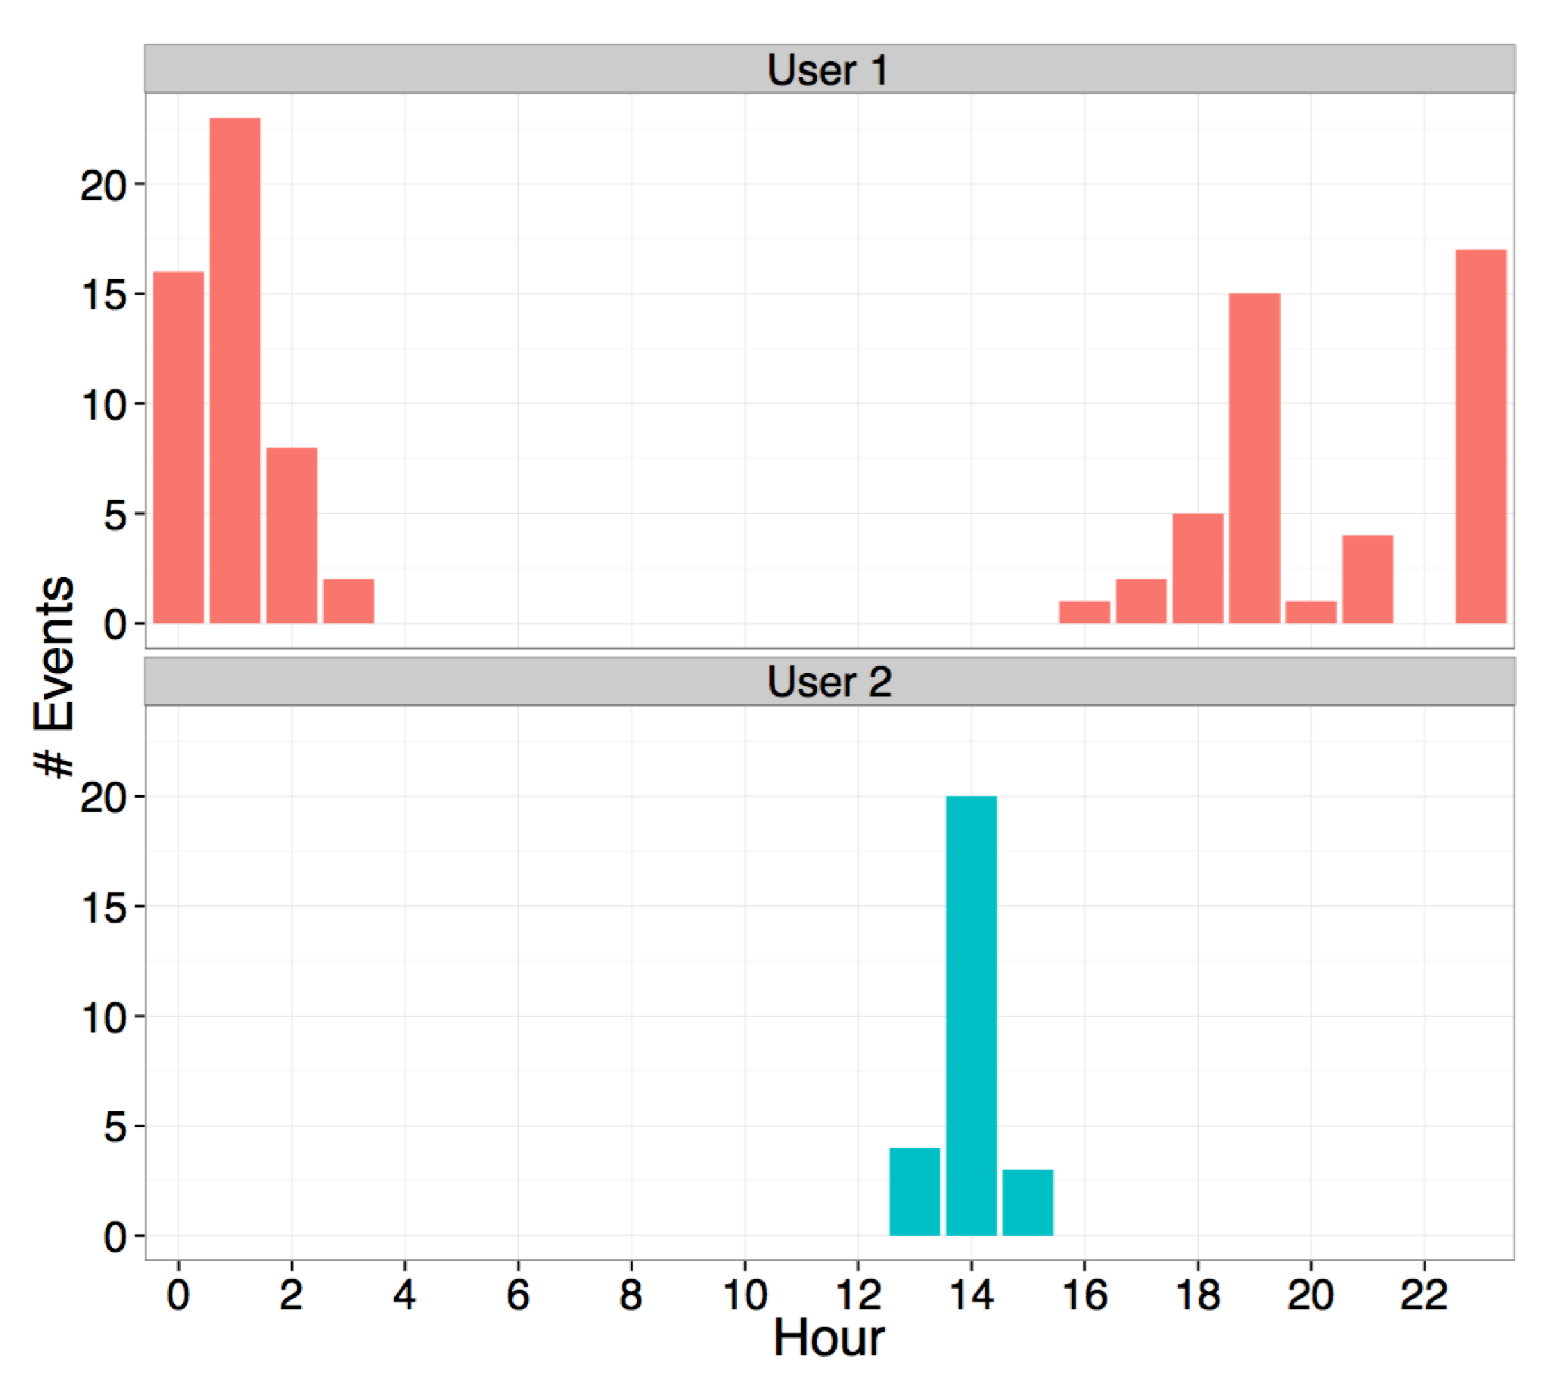
\includegraphics[width=0.7\columnwidth]{figs/figsss/14.eps}}
\end{figure}
}

\frame{\frametitle{Which day do users go to events?}
\begin{figure}[h]
\centering
{\includegraphics[width=0.75\columnwidth]{figs/figsss/15.eps}}
\end{figure}
}

\frame{\frametitle{Time-Aware}
Each user is the centroid of the events she attended in the past:

$$\vec{u} := \frac{1}{E_u}\sum\limits_{e\in E_u}\vec{e}.$$

where $\vec{e}$ is a $24 \times 7$-dimensional vector in the space of all possible days of the week and hours of the day. \\
\vspace{0.5cm}
The recommendation score is now:
$$\hat{s}(u, e) := cos(\vec{u}, \vec{e})$$
}


\subsection{Location-Aware}

\frame{\frametitle{Location-Aware}
{\color{blue}Assumption}: Users tend to attend events close to the events they
attended in the past.
\begin{columns}
\column{0.5\textwidth}
\begin{figure}[h]
\centering
\subfigure[User 1]
{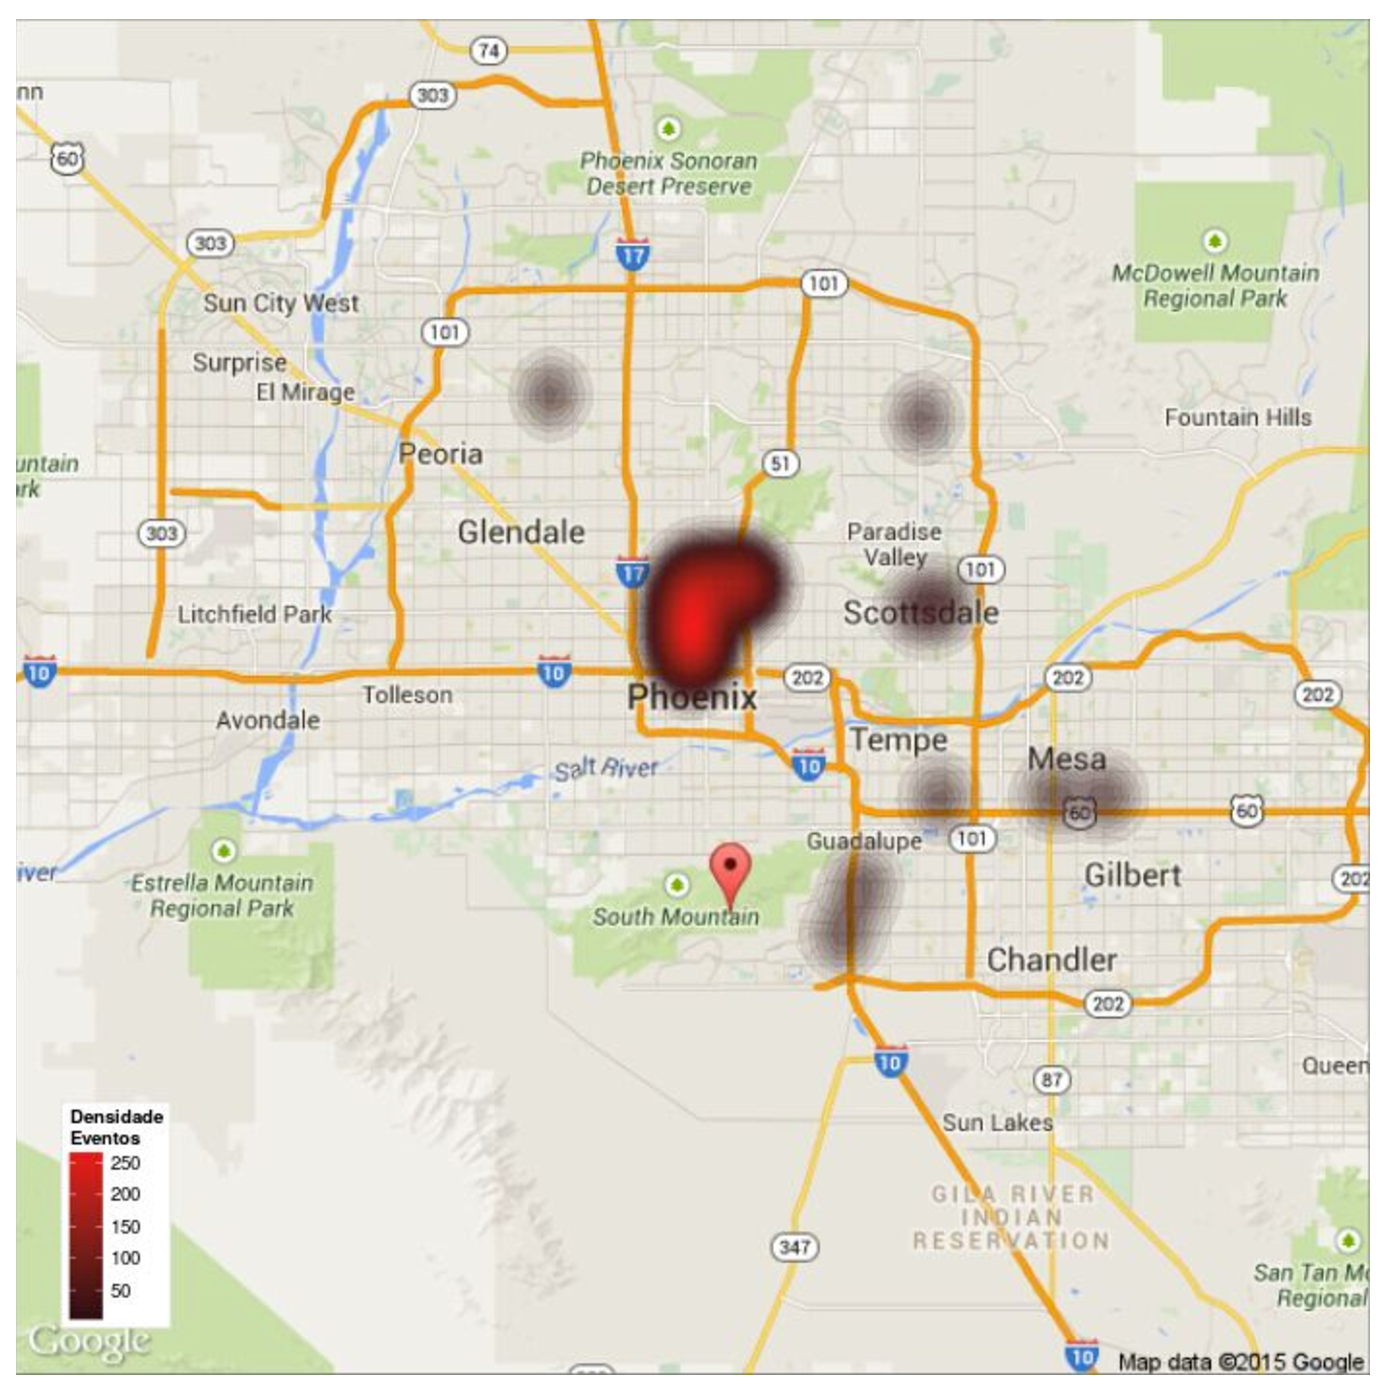
\includegraphics[width=0.8\columnwidth]{figs/6.eps}}
\end{figure}

\column{0.5\textwidth}
\begin{figure}[h]
\centering
\subfigure[User 2]
{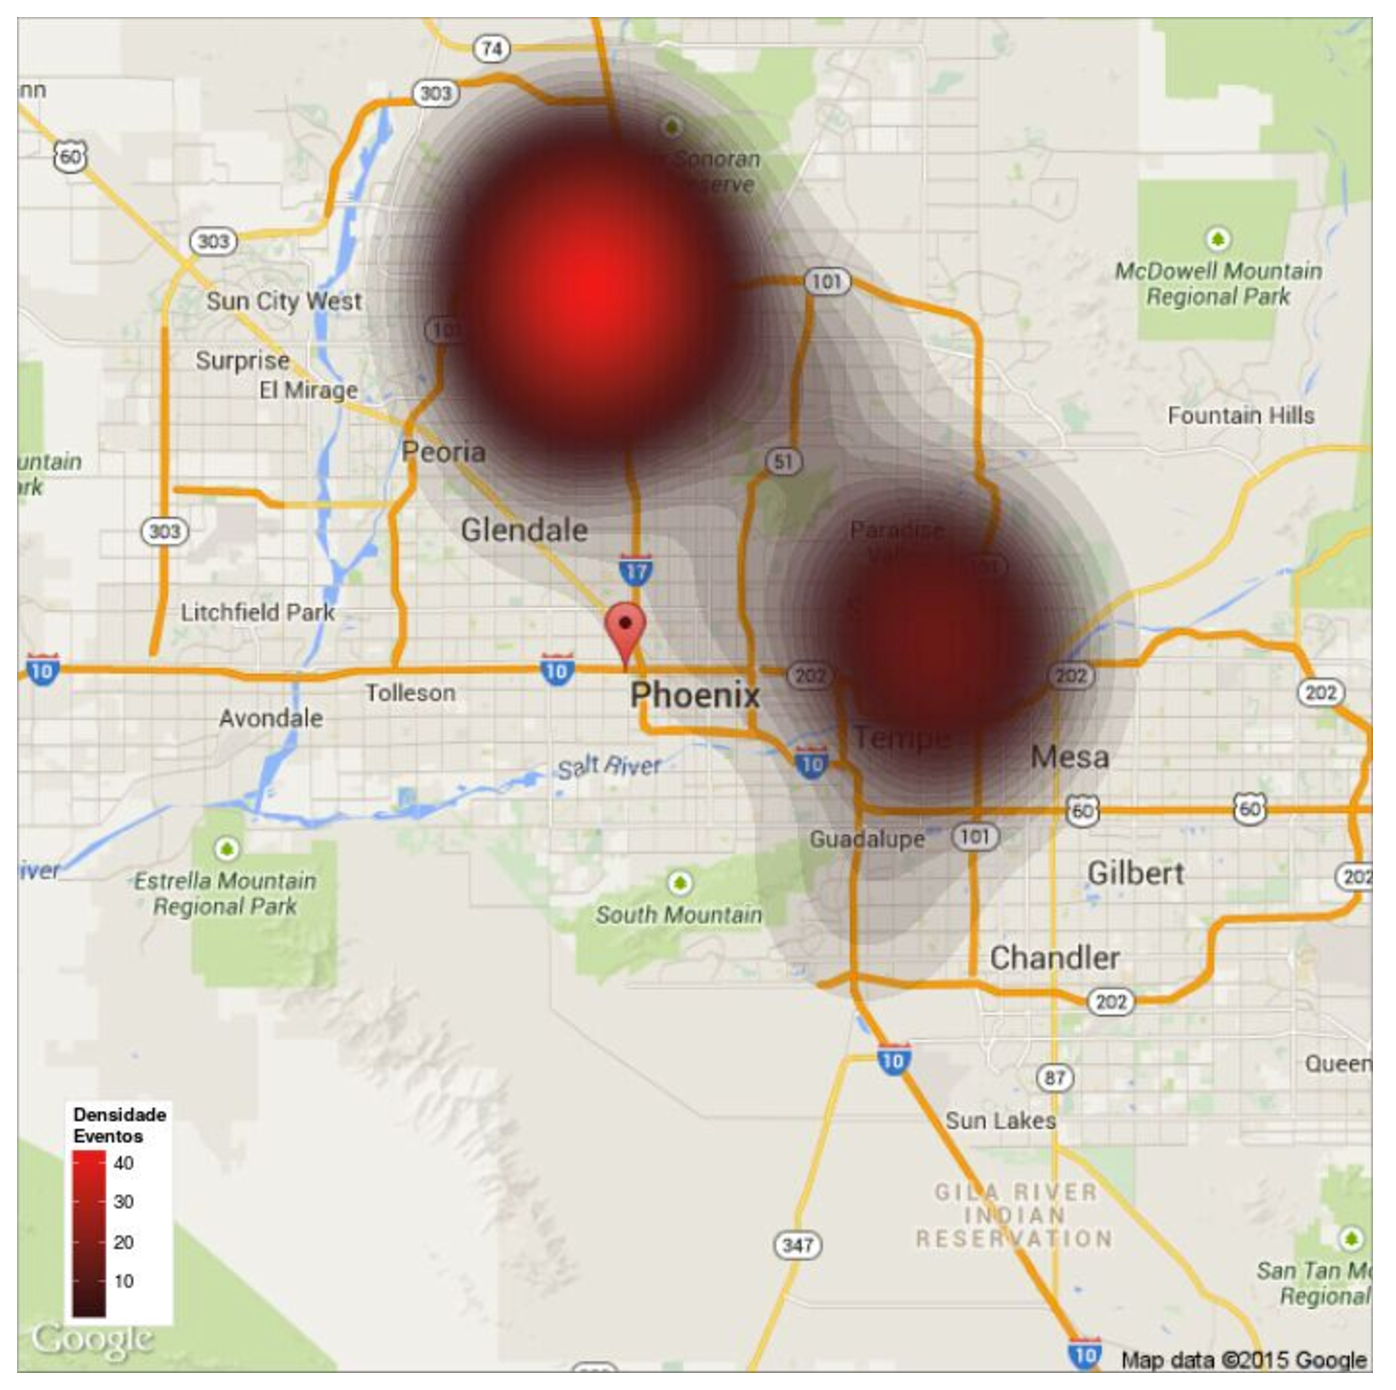
\includegraphics[width=0.8\columnwidth]{figs/7.eps}}
\end{figure}
\end{columns}
}

\frame{\frametitle{Kernel Density Estimation}
The recommendation score is given by
$$\hat{s}(u,e) = \frac{1}{|L_u|}\sum\limits_{l' \in L_u}K_H(l_e - l').$$
where $l_e$ is the lat-long coordinate of event e and $K_H$ is the Gaussian kernel.
}


\subsection{Learning to Rank}
\frame{\frametitle{Learning to Rank}
Let $\mathcal{D} := \{(x_1, y1), \ldots, (x_n, y_n)\}$ be the training set where $x_i := (\hat{s_1}(u, e)$,
$\ldots, \hat{s_m}(u,e), |U_e|)$ is a feature vector containing the scores for each recommender and $y_i = \{0,1\}$ denote whether user $u$ attended event $e$ or not. \\
\vspace{0.5cm}

The goal is to learn a function $h(x)$ s.t. for any pair $(x_i, y_i)$ and $(x_j, y_j)$ the following holds:
$$h(x_i) > h(x_j)  \Leftrightarrow y_i > y_j.$$
\vspace{0.1cm}

We have used \textbf{Coordinate Ascent} [Metzler, 2007], a state-of-the-art listwise learning to rank approach.
}


\section{Evaluation}

\subsection{Research Questions}

\frame{\frametitle{Research Questions}
\begin{enumerate}
\item[$Q1.$] How \textbf{effective} is MCLRE for event recommendation?
\pause
\item[$Q2.$] How \textbf{robust} is MCLRE to \textbf{sparsity} in the RSVP data?
\pause
\item[$Q3.$] Which contextual \textbf{features} are \textbf{effective} recommenders?
\end{enumerate}
}


\subsection{Data Collection}
\frame{\frametitle{Evaluation Protocol}
\begin{itemize}
\item Meetup.com data from January, 2010 to April, 2014
\item Cities Collected: Phoenix, Chicago and San Jose
\end{itemize}

\vspace{0.3cm}

\begin{table}[htbp]
\centering  % ������
\begin{tabular}{c|c|c|c|c|c}
\textbf{City} & $|G|$ & $|U|$ & $|E|$ & \textbf{RSVPs} & \textbf{Sparsity} \\ \hline
Chicago       & 2,321 & 207,649 & 190,927 & 1,375,154 & 99.99\% \\ \hline
Phoenix       & 1,661 & 117,458 & 222,632 & 1,209,324 & 99.95\% \\ \hline
San Jose      & 2,589 & 242,143 & 206,682 & 1,607,985 & 99.99\% \\ \hline
\end{tabular}
\end{table}
}


\subsection{Evaluation Protocol}
\frame{\frametitle{Evaluation Protocol}
\begin{itemize}
\item 12 time stamps equally spaced in time over 52 months.
\item Sliding training window.
\item For each city, the four initial partitions are used as validation sets and the remaining partitions for evaluation.
\end{itemize}
\begin{figure}[h]
\centering
{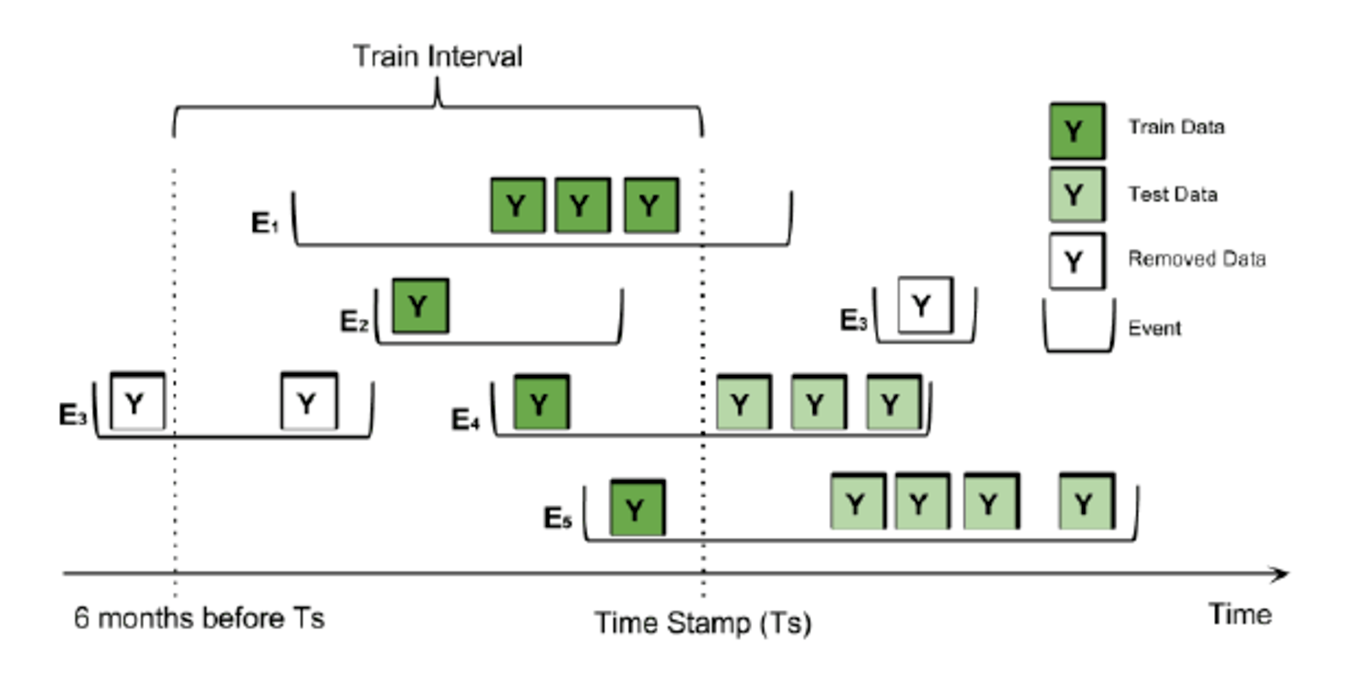
\includegraphics[width=0.80\columnwidth]{figs/figsss/1312.eps}}
\end{figure}
}


\subsection{Compared Algorithm}
\frame{\frametitle{Compared Algorithm}
\begin{itemize}
\item Most Popular
\item BPR-MF [Rendle, 2009]
\item BPR-NET [Qiao, 2014]
\item \textbf{MCLRE}
\item Evaluation Metric: NDCG@10
\end{itemize}
}

\subsection{Recommendation Effectiveness}

\frame{\frametitle{Recommendation Effectiveness}
\begin{figure}[h]
\centering
{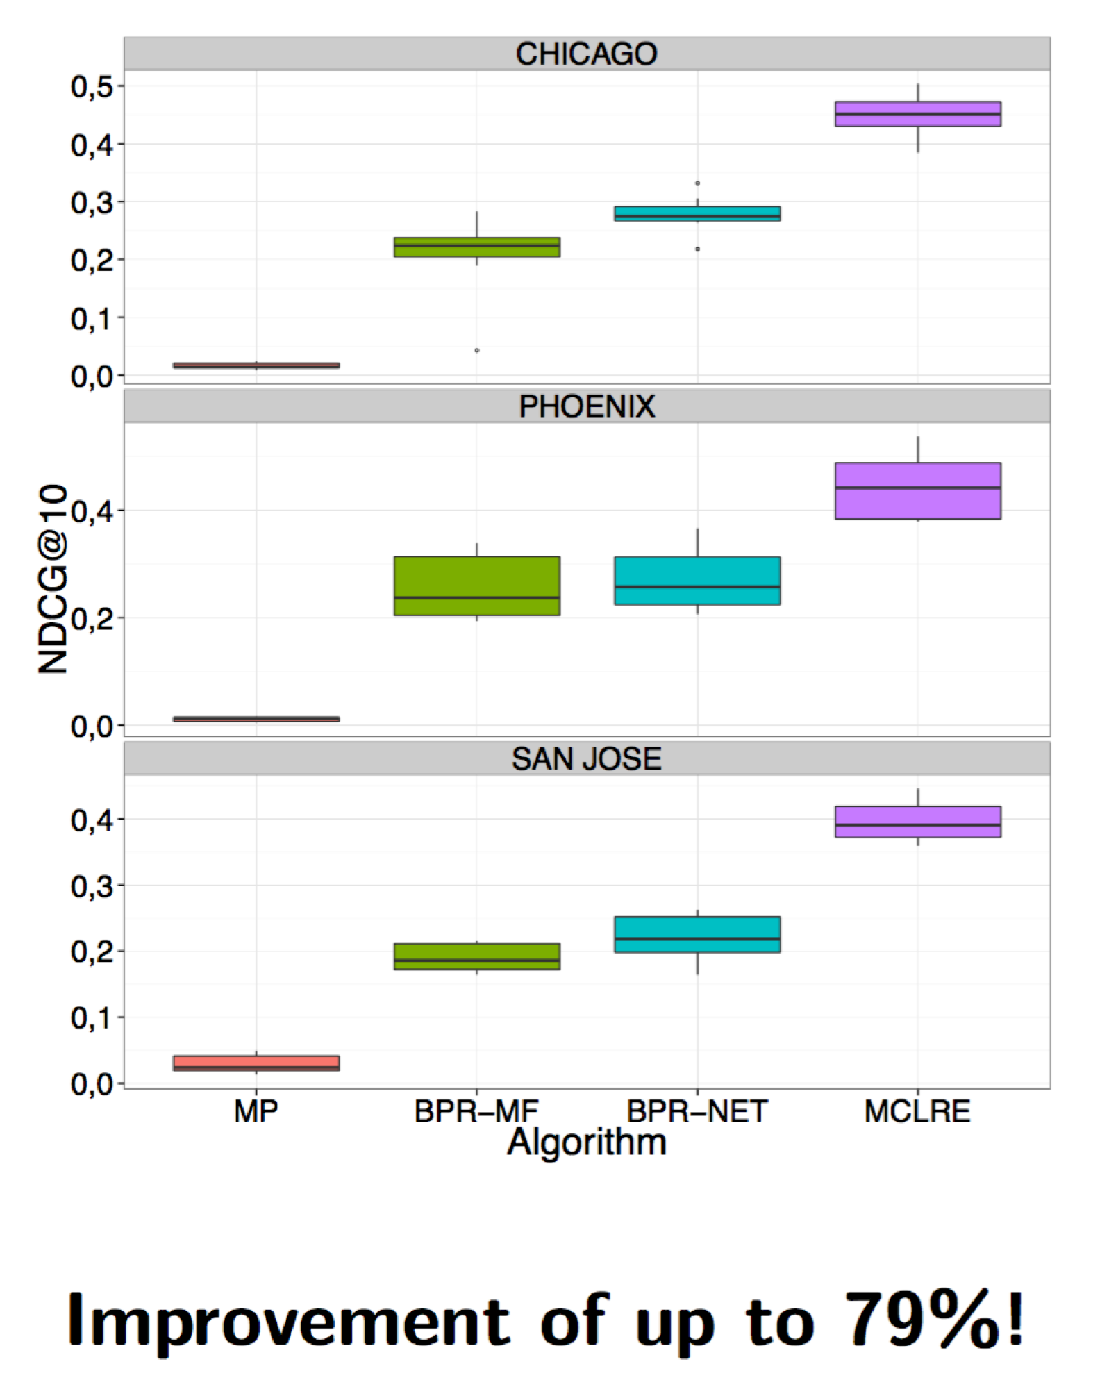
\includegraphics[width=0.50\columnwidth]{figs/figsss/16.eps}}
\end{figure}
}

\subsection{Robustness to Data Sparsity}
\frame{\frametitle{Robustness to Data Sparsity}
\begin{figure}[h]
\centering
{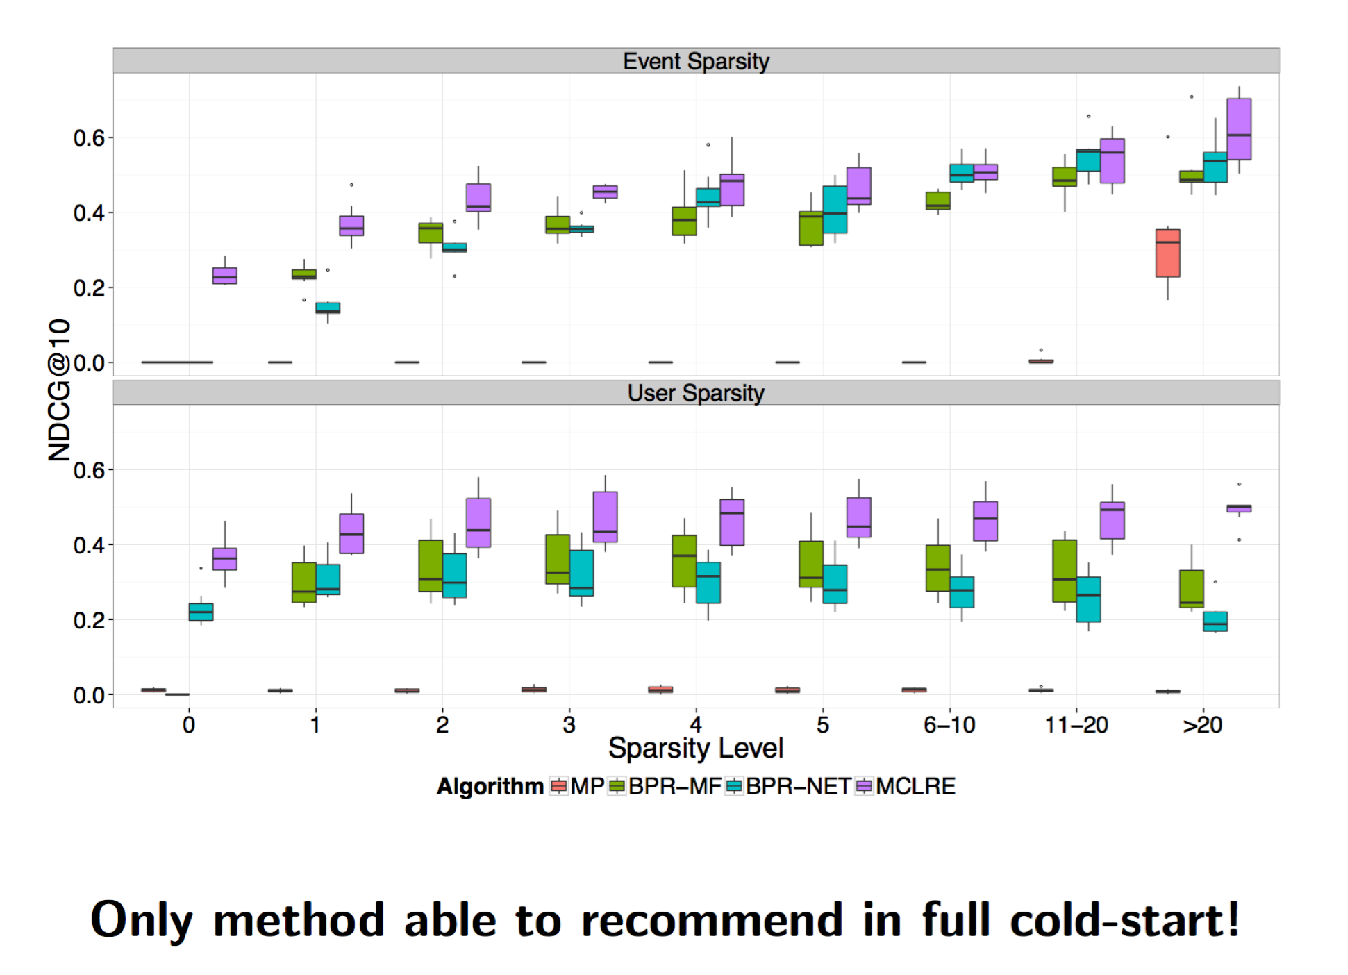
\includegraphics[width=0.86\columnwidth]{figs/figsss/17.eps}}
\end{figure}
}

\subsection{Contextual Feature Analysis}
\frame{\frametitle{Contextual Feature Analysis}
\begin{figure}[h]
\centering
{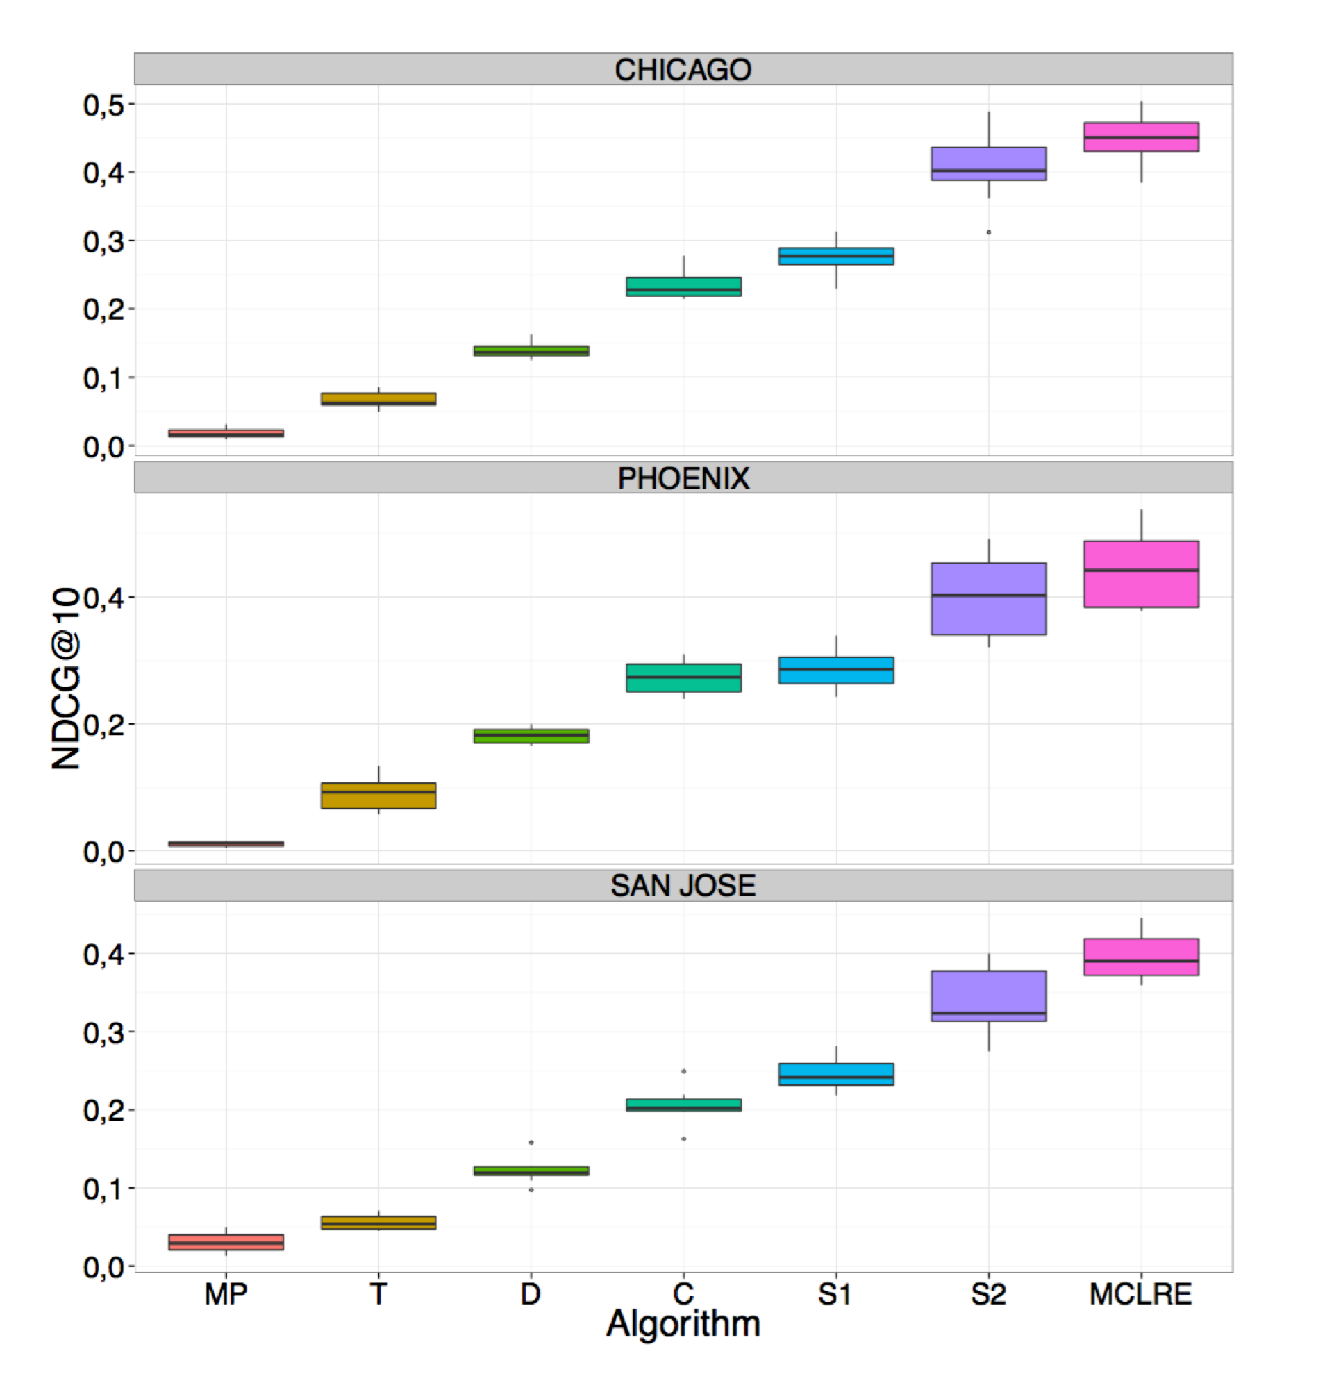
\includegraphics[width=0.58\columnwidth]{figs/figsss/18.eps}}
\end{figure}
}

\section{Conclusions}

\frame{\frametitle{Conclusions}
\begin{itemize}
\item The use of multiple contexts can both lead to highly accurate
recommendations and mitigate the cold-start problem.
\vspace{0.8cm}
\item Events created by groups of which a user is a member are far
more relevant than the content of the events or collaborative
RSVP data.
\end{itemize}
}

\end{CJK}
\end{document}
